\documentclass[11pt,letterpaper]{article}
\usepackage[lmargin=1in,rmargin=1in,tmargin=1in,bmargin=1in]{geometry}
\usepackage{../style/homework}
\usepackage{../style/commands}
\setbool{quotetype}{true} % True: Side; False: Under
\setbool{hideans}{false} % Student: True; Instructor: False

% -------------------
% Content
% -------------------
\begin{document}

\homework{1: Due 01/25}{I mean not homework. It's not work if you love it.}{Alex Dunphy, Modern Family}

% Problem 1
\problem{10} \textit{High Voltage} is an electronics store that, among other products, sells televisions. They sell a particular brand of OLED TV that costs \$949.99. To help drive up sales, they will place the TV on sale for 15\% off. 
	\begin{enumerate}[(a)]
	\item What is the mark-down on this television, i.e. what is the discount?
	\item What is the final advertised price for the television?
	\item How much is the TV after a sales tax of 7\%. 
	\item Suppose over next two months, they discount the price by 15\% twice, what is the advertised price of the television? 
	\end{enumerate} \pspace

\sol 
\begin{enumerate}[(a)]
\item The markdown, i.e. discount, is 15\% of \$949.99. But this is $\$949.99(0.15) \approx \$142.50$. \pspace

\item From (a), we know that the product has been marked down by \$142.50. But then the final price is $\$949.99 - \$142.50= \$807.49$. Alternatively, because the TV is on sale for 15\% off, only $100\% - 15\%= 85\%$ of the cost remains. But this is $\$949.99 (0.85) \approx \$807.50$. \pspace

\item From (b), the discounted price is \$807.50. But then this is increased by 7\% due to sales tax. Therefore, the final price is $\$807.50 (1 + 0.07)= \$807.50(1.07) \approx \$864.03$. \pspace

\item Each time the TV is discounted by 15\%, only 85\% of its price remains. But then the cost of the TV is\dots
	\[
	\$807.50 (0.85)(0.85)= \$807.50 (0.85)^2= \$807.50 (0.7225) \approx \$583.42
	\]
From the computation above, we can see that in the end it is as if the TV is discounted by another 27.75\% (because $0.7225= 1 - 0.2775$). [Note: This is equivalent to its original price being discounted by approximately 38.59\% because $(0.85)^3= 0.614125$ and $0.614125= 1 - 0.385875$.]
\end{enumerate}



\newpage



% Problem 2
\problem{10} Suppose that Richard Hoover is driving across the Southwest. After a day of driving, he maps out his travel plans over the next few days. He predicts that the total number of miles he will drive $d$ days from now is given by $M(d)= 390d + 135$. 
	\begin{enumerate}[(a)]
	\item What is the slope of $M(d)$? What does it represent?
	\item What is the $y$-intercept of $M(d)$? What does it represent?
	\item On the plot below, sketch $M(d)$. 
	\item Find how many miles he will have driven after 3 total days of driving.
	\end{enumerate} \pspace

\sol 
\begin{enumerate}[(a)]
\item The function $M(d)= 390d + 135$ is a linear function because it has the form $y= mx + b$ with $M= y$, $d= x$, $m= 390$, and $b= 135$. Therefore, the slope of $M(d)$ is 390. Interpreting this slope $m= 390= \frac{390}{1}$ as $m= \frac{\Delta M}{\Delta t}$, we see that for each additional day, Richard has driven an additional 390~miles; that is, Richard is driving 390~miles each day. \pspace

\item From (a), we can see that the $y$-intercept is 135; that is, $M(0)= 135$. But then after 0 additional days after his first day of driving, Richard has driven 135~miles; that is, Richard drove 135~miles on his first day. \pspace

\item We know that $M(d)= 390d + 135$ is a line with $y$-intercept 135 and slope $390$. We can see the sketch of the function on the graph below. \pspace

\item This is $M(3)= 390(3) + 135= 1170 + 135= 1305$. Therefore, Richard has driven a total of 1305~miles after 4 days (3 additional days after his first day). 
\end{enumerate} \vfill


	\[
	\fbox{
	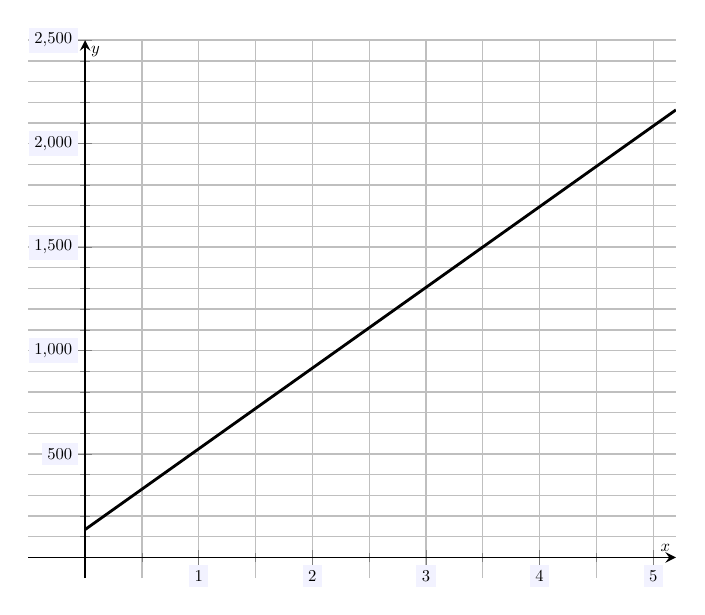
\begin{tikzpicture}[scale=1.2,every node/.style={scale=0.5}]
	\begin{axis}[
	grid=both,
	axis lines=middle,
	ticklabel style={fill=blue!5!white},
	xmin= -0.5, xmax=5.2,
	ymin= -100, ymax=2500,
	xtick={0,1,2,3,4,5},
	ytick={0,500,1000,...,2500},
	minor x tick num = 1,
	minor y tick num = 4,
	xlabel=\(x\),ylabel=\(y\),
	]
	\addplot[domain=0:5.2,samples=2,line width=0.03cm] (x, 390*x + 135);
	\end{axis}
	\end{tikzpicture}
	}
	\] 


\end{document}